\documentclass[10pt]{beamer}

\usepackage{polyglossia}
\usepackage{csquotes}
\usepackage{datetime}
\usepackage{fontspec}
\usepackage{microtype}
\usepackage{color}
\usepackage{url}
\usepackage{hyperref}
\usepackage{amsfonts}
\usepackage{amsmath}
\usepackage{amsthm}
\usepackage{subcaption}
\usepackage[backend=biber,style=iso-authoryear,sortlocale=en_US,autolang=other,bibencoding=UTF8]{biblatex}
\usepackage{booktabs}
\usepackage{graphics}
\usepackage{pifont}
\usepackage{tikz}

\addbibresource{zotero.bib}

\setdefaultlanguage{czech}
\setotherlanguage{english}
\usefonttheme{professionalfonts}
\setmainfont{TeX Gyre Termes}
\usetheme{Boadilla}
\usecolortheme{crane}
\setbeamertemplate{title page}[default][rounded=true,shadow=false]
\setbeamertemplate{section in toc}[ball unnumbered]
\setbeamertemplate{bibliography item}{}

\hypersetup{
	pdfencoding=auto,
	unicode=true,
	citecolor=green,
	filecolor=blue,
	linkcolor=red,
	urlcolor=blue
}

\makeatletter
\newcommand*{\currentSection}{\@currentlabelname}
\makeatother

\title[Learning on graph-structured data]
{
	Learning on graph-structured data
}

%\newdate{presentation}{06}{11}{2020}
%\date{\displaydate{presentation}}
\date[6. 11. 2020]{6. listopadu 2020}

\author[Marek Dědič]
{
	Marek~Dědič\inst{1}
}

\institute[FJFI ČVUT]
{
	\inst{1} ČVUT v Praze, Fakulta jaderná a fyzikálně inženýrská
}

\AtBeginSection[]{
	\begin{frame}{\currentSection}
		\tableofcontents[currentsection]
	\end{frame}
}

\newcommand{\mathvec}{\ensuremath{\mathbf}}
\newcommand{\mathmat}{\ensuremath{\mathbf}}
\newcommand{\mathspace}{\ensuremath{\mathcal}}
\newcommand{\mathfield}{\ensuremath{\mathbb}}

\begin{document}

\begin{frame}
	\titlepage
\end{frame}

\begin{frame}{Obsah}
	\tableofcontents
\end{frame}

% Body

\section{Motivace}

\begin{frame}{Motivace}
	\begin{itemize}
		\item Grafy jsou přirozenou abstrakcí pro mnoho matematických úloh
		\item Využití v chemii, softwarovém inženýrství, zpracování obrazu, medicíně, částicové fyzice, síťové bezpečnosti, detekce fake-news, autonomních vozidlech...
	\end{itemize}
	\centering
	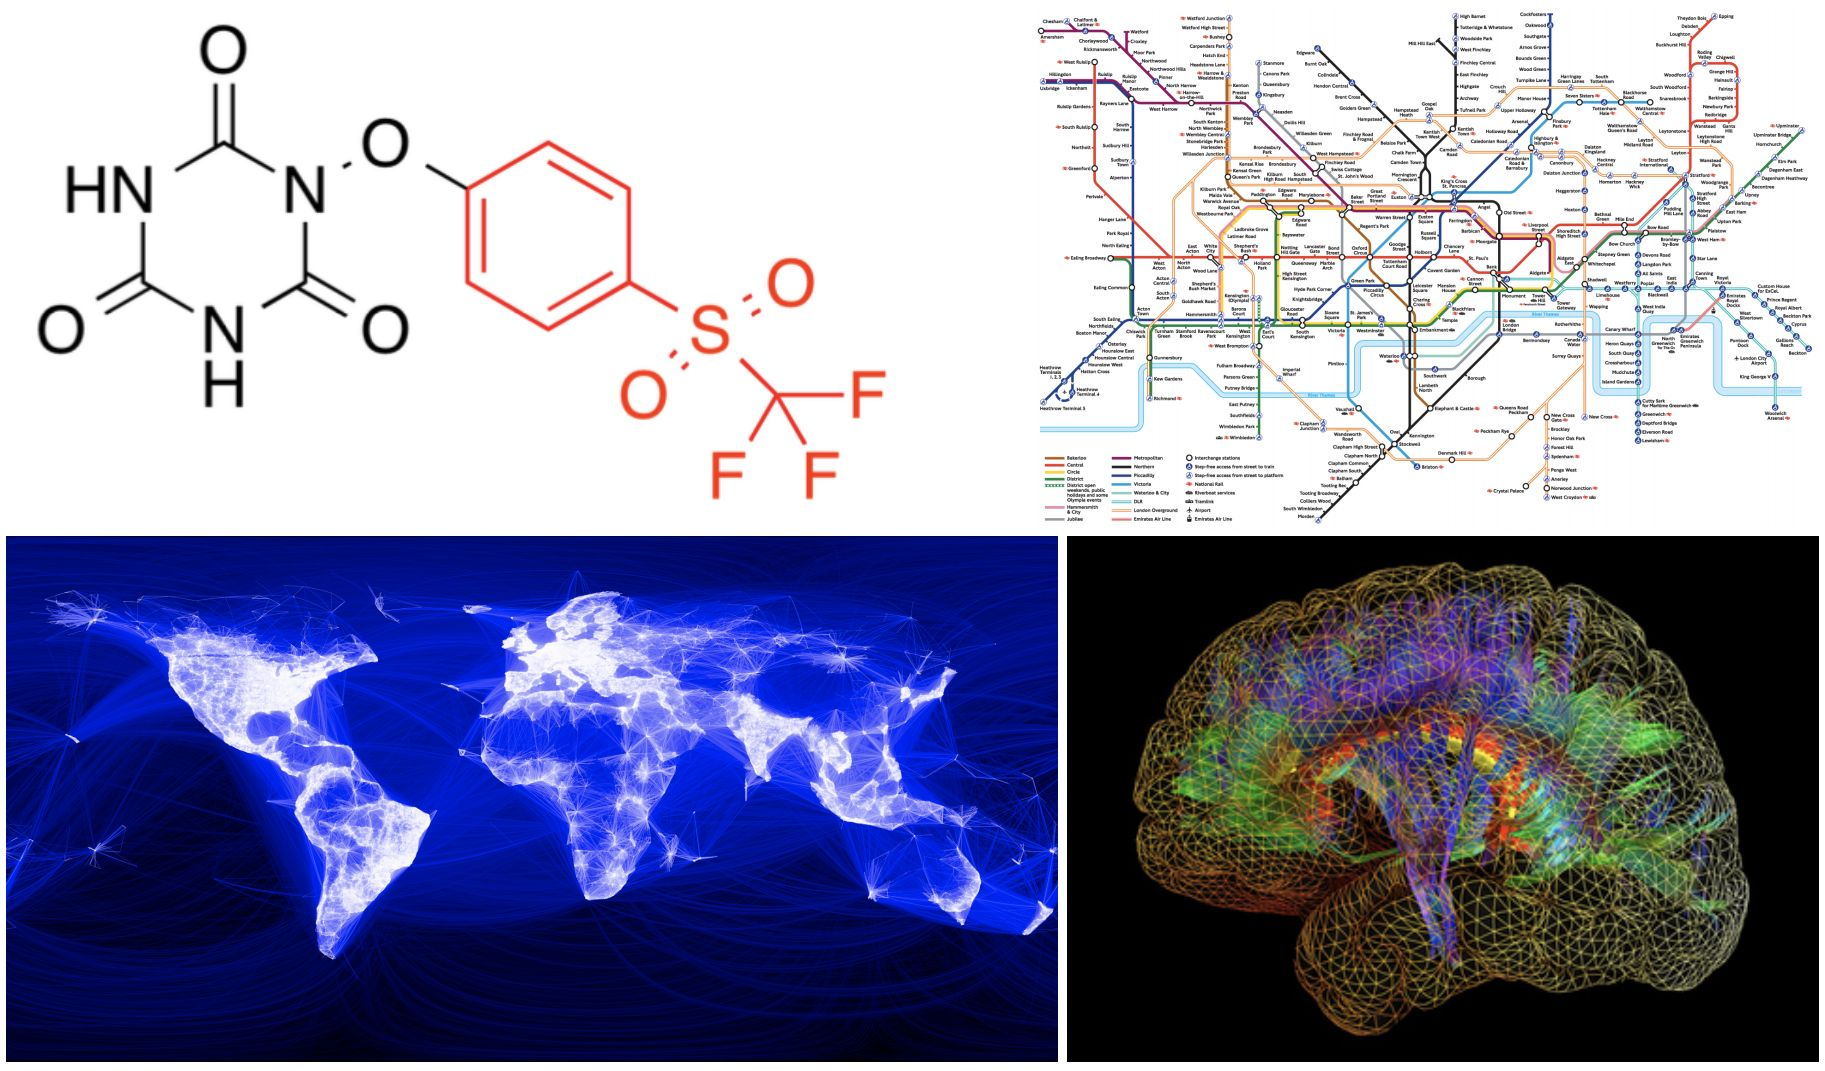
\includegraphics[width=0.7\pagewidth]{images/graphs.png}\footnote{\cite{velickovic_opening_2020}}
\end{frame}

\begin{frame}{Definice}
	\begin{itemize}
		\item Graf \( G = \left( V, E \right) \)
		\item \( ne \left[ v \right] \) je množina vrcholů, ze kterých vede hrana do \( v \).
		\item \( co \left[ v \right] \) je množina hran vedoucích z nebo do \( v \).
		\item \( x_v \) jsou příznaky vrcholu \( v \).
		\item \( x_e \) jsou příznaky hrany \( v \).
	\end{itemize}
\end{frame}

\section{Úlohy}

\begin{frame}{Node classification}
	\centering
	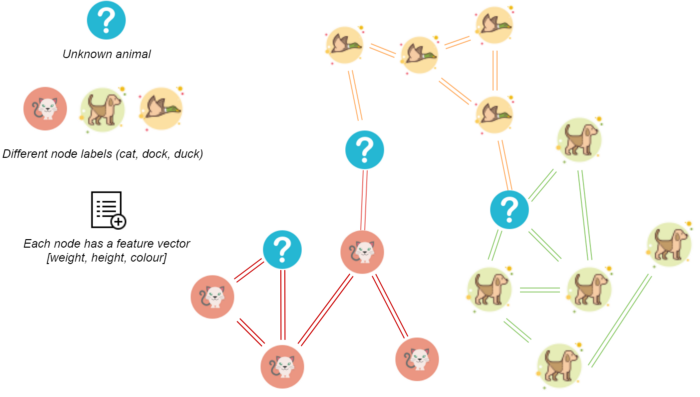
\includegraphics[width=0.7\pagewidth]{images/node-classification.png}\footnote{\cite{kubara_machine_2020}}
\end{frame}

\begin{frame}{Link prediction}
	\centering
	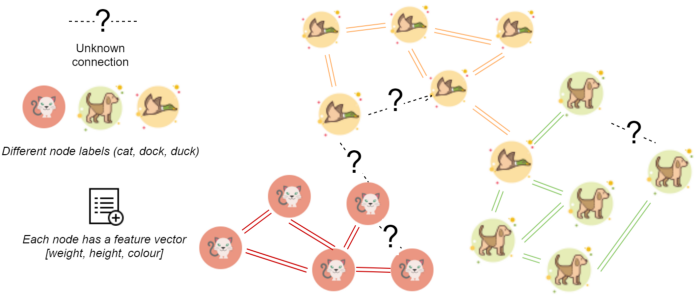
\includegraphics[width=0.7\pagewidth]{images/link-prediction.png}\footnote{\cite{kubara_machine_2020}}
\end{frame}

\begin{frame}{Učení se na celém grafu}
	\centering
	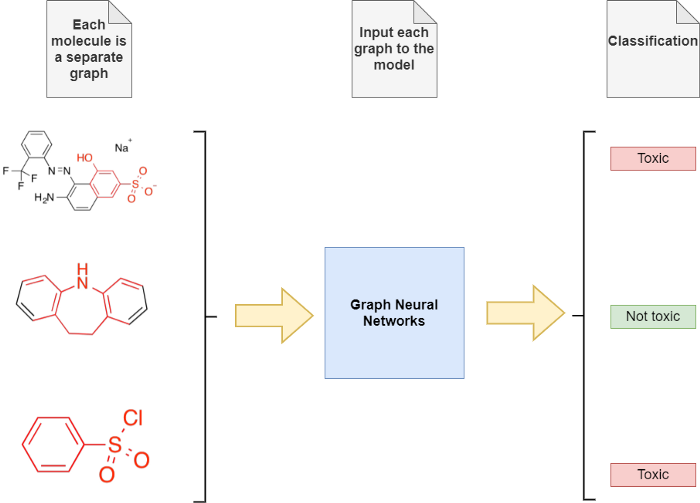
\includegraphics[width=0.7\pagewidth]{images/whole-graph-learning.png}\footnote{\cite{kubara_machine_2020}}
\end{frame}

\begin{frame}{Community detection}
	\centering
	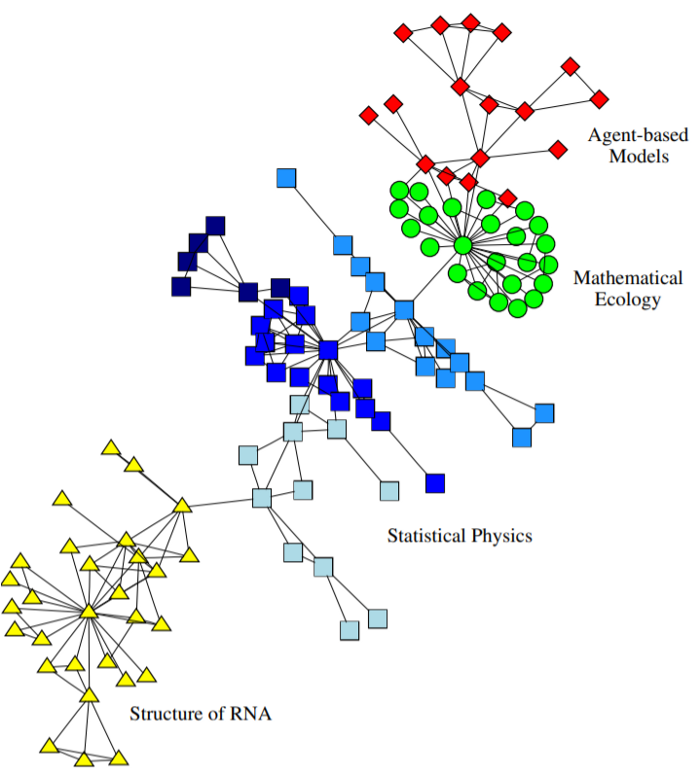
\includegraphics[width=0.5\pagewidth]{images/community-detection.png}\footnote{\cite{girvan_community_2002}}
\end{frame}

\section{GNN}

\begin{frame}{GNN 1}
	\begin{itemize}
		\item Řešíme úlohu \enquote{Node classification}.
		\item Adaptace neuronových sítí na grafová data
		\item Formálně klasifikace na prostoru \( \mathspace{G} \times \mathspace{N} \) - páry graf + jeden jeho vrchol
		\item Předpokládáme pro každý vrchol \( v \) a hranu \( e \) příznaky \( \mathvec{x}_v \) a \( \mathvec{x}_e \).
		\item Modelujeme pro každý vrchol \( v \) skrytý stav \( \mathvec{h}_v \) zachycující informaci o \( v \) a jeho okolí.
	\end{itemize}
\end{frame}

\begin{frame}{GNN 2}
	\begin{itemize}
		\item Modelujeme pro každý vrchol \( v \) skrytý stav \( \mathvec{h}_v \) zachycující informaci o \( v \) a jeho okolí jako
			\[ \mathvec{h}_v = f \left( \mathvec{x}_v, \mathvec{x}_{co \left[ v \right]}, \mathvec{h}_{ne \left[ v \right]}, \mathvec{x}_{ne \left[ v \right]} \right) \]
		\item ...a výstup pro vrchol \( v \) jako
			\[ \mathvec{o}_v = g \left( \mathvec{h}_v, \mathvec{x}_v \right) \]
		\item Můžeme skrytý stav \( \mathvec{h}_v \) počítat dohromady pro všechny vrcholy iterativně jako
			\[ \mathmat{H}^{t + 1} = F \left( \mathmat{H}^t, \mathmat{X} \right) \]
	\end{itemize}
\end{frame}

\begin{frame}{GNN 3}
	\centering
	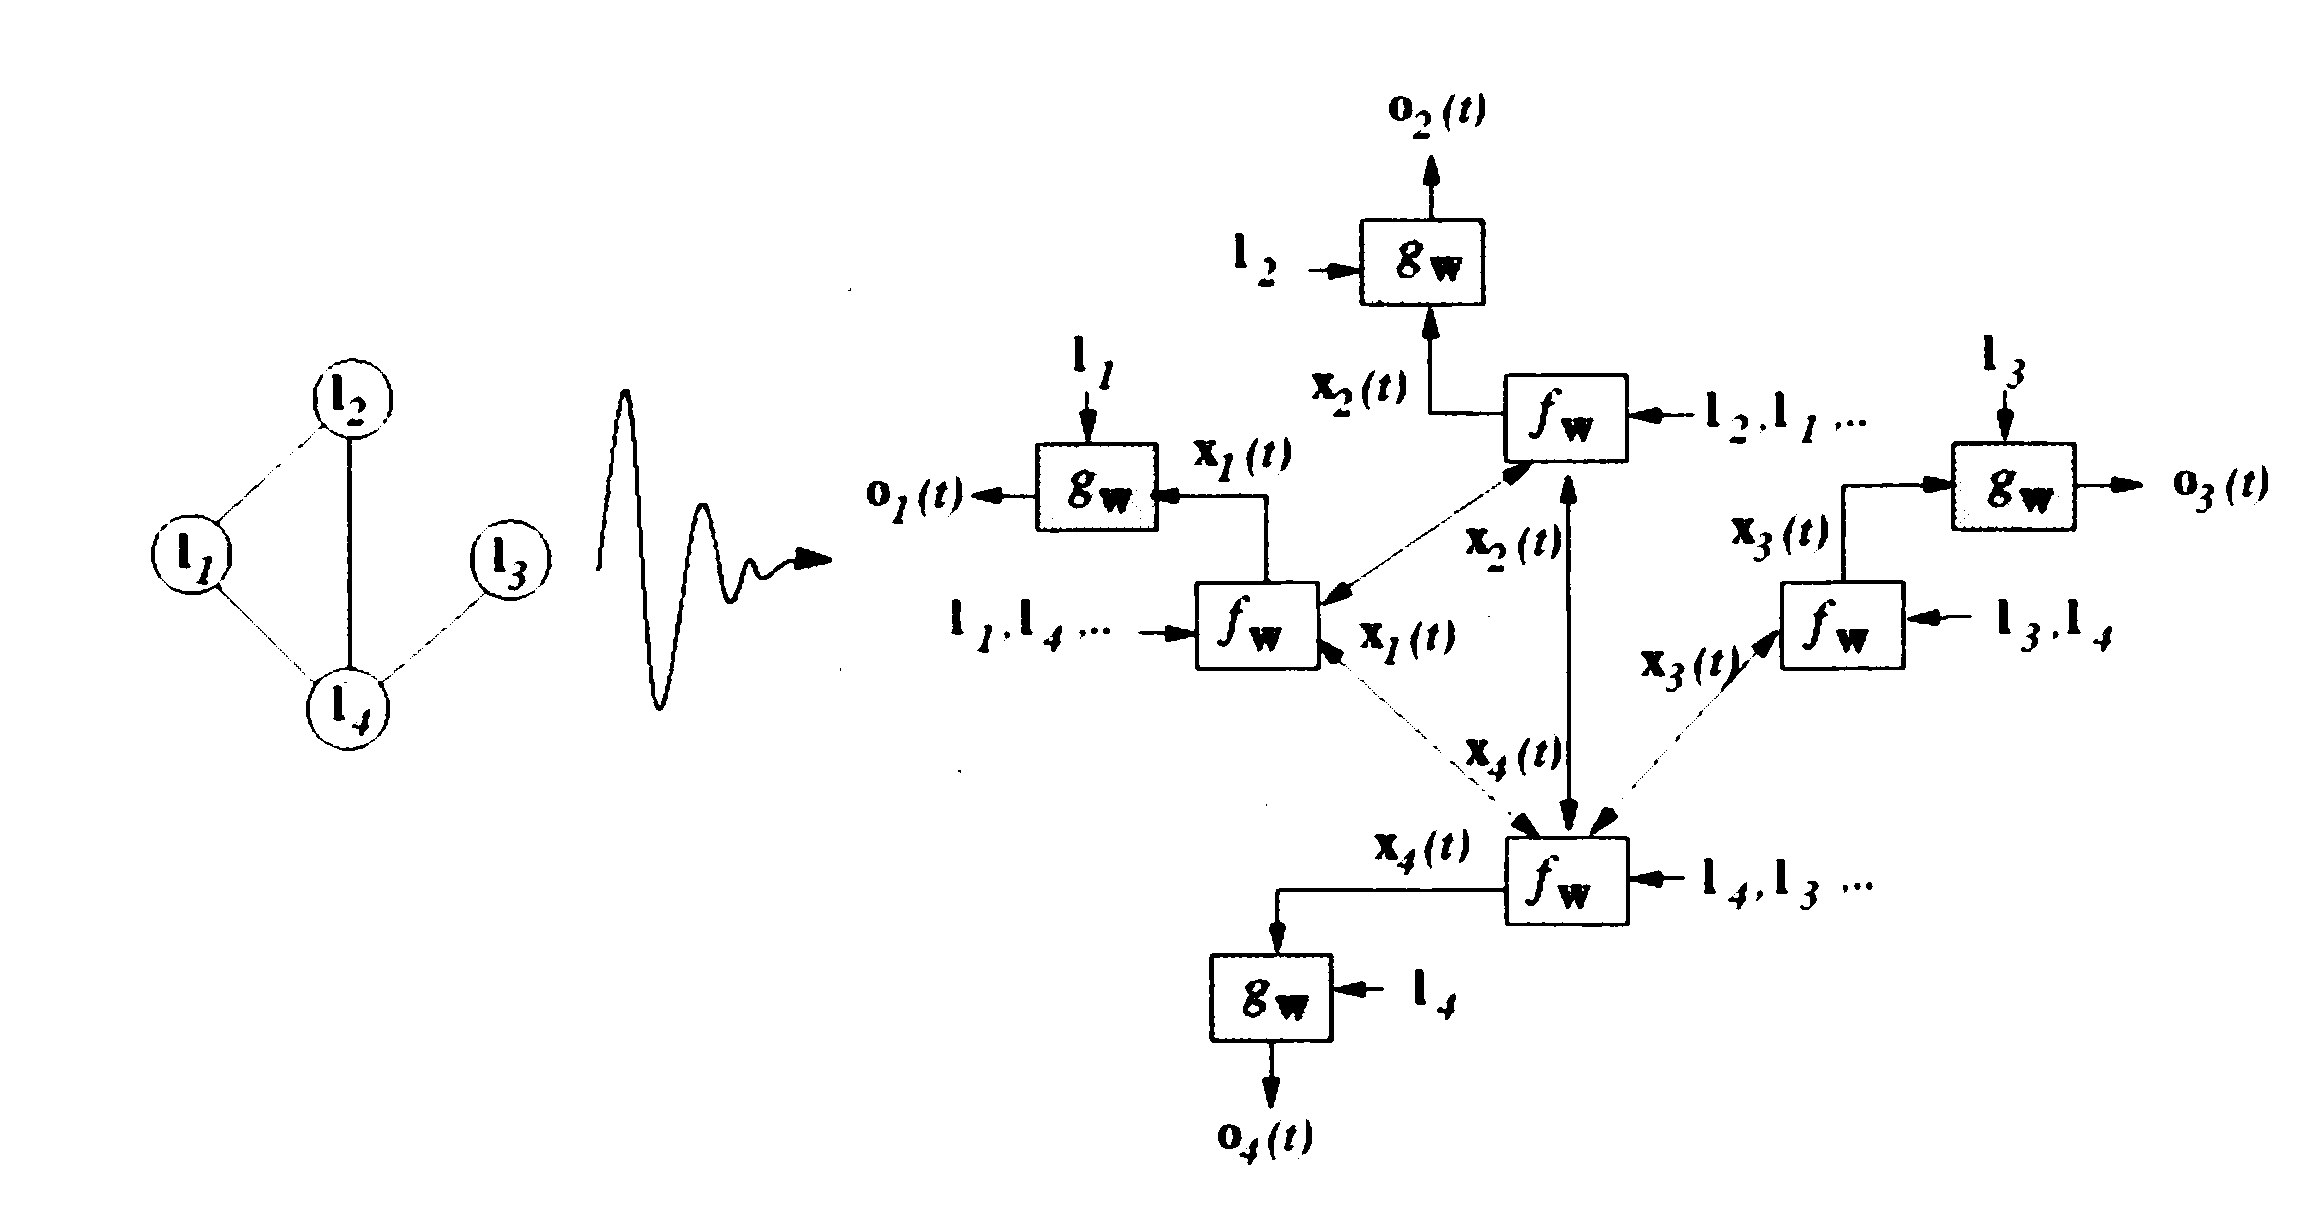
\includegraphics[width=0.9\pagewidth]{images/GNN.png}\footnote{\cite{gori_new_2005}}
\end{frame}

\begin{frame}{GNN -- závěr}
	\begin{itemize}
		\item Na iterativní opakování aplikace funkce \( F \) lze nahlížet jako na RNN.
		\item Lze nahradit iterativní proces za MLP.
		\item Nepoužívány skryté stavy hran, pouze vrcholů
	\end{itemize}
\end{frame}

\begin{frame}{GNN -- modifikace}
	\begin{figure}[h]
		\centering
		\begin{subfigure}[t]{0.33\textwidth}
			\centering
			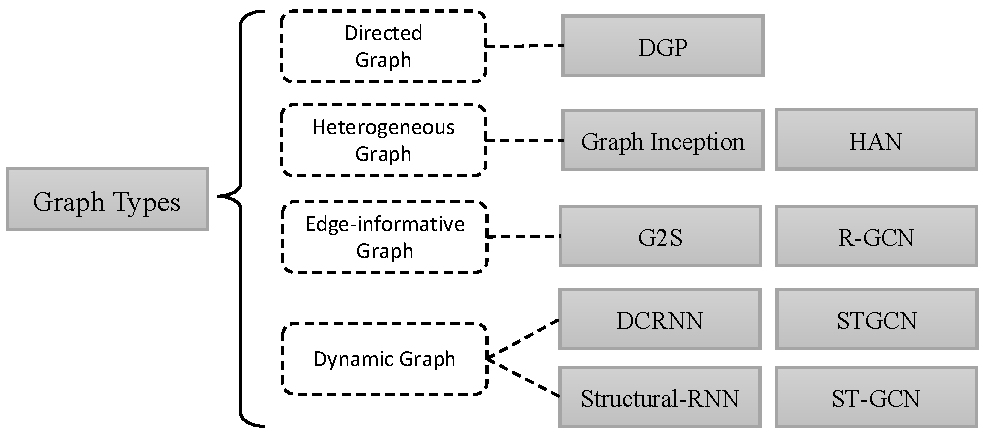
\includegraphics[width=1\linewidth]{images/GNN-variants/variant1.pdf}
		\end{subfigure}
		\begin{subfigure}[t]{0.43\textwidth}
			\centering
			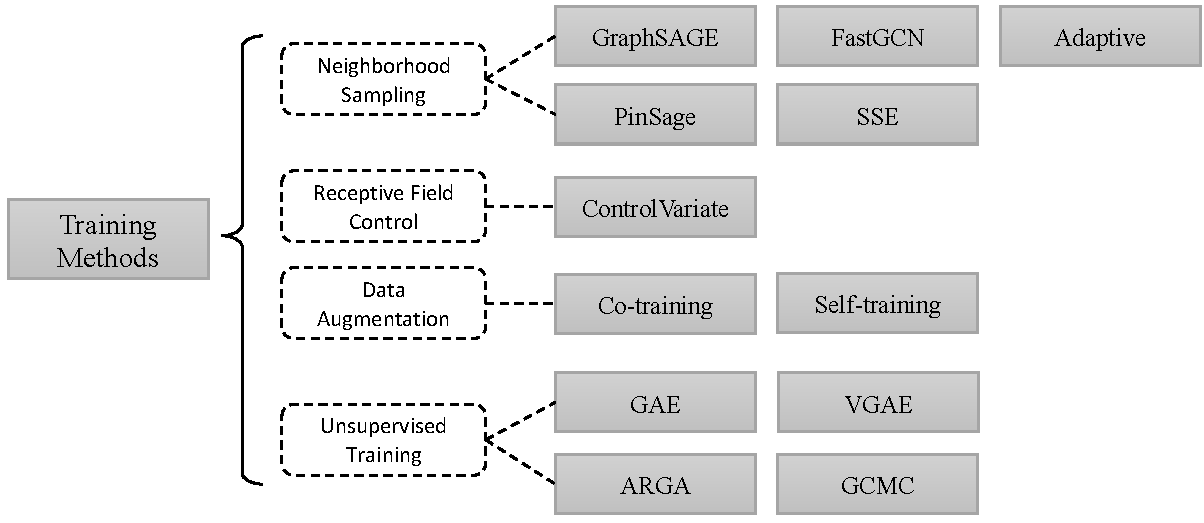
\includegraphics[width=1\linewidth]{images/GNN-variants/variant3.pdf}
		\end{subfigure}
		\begin{subfigure}[t]{0.65\textwidth}
			\centering
			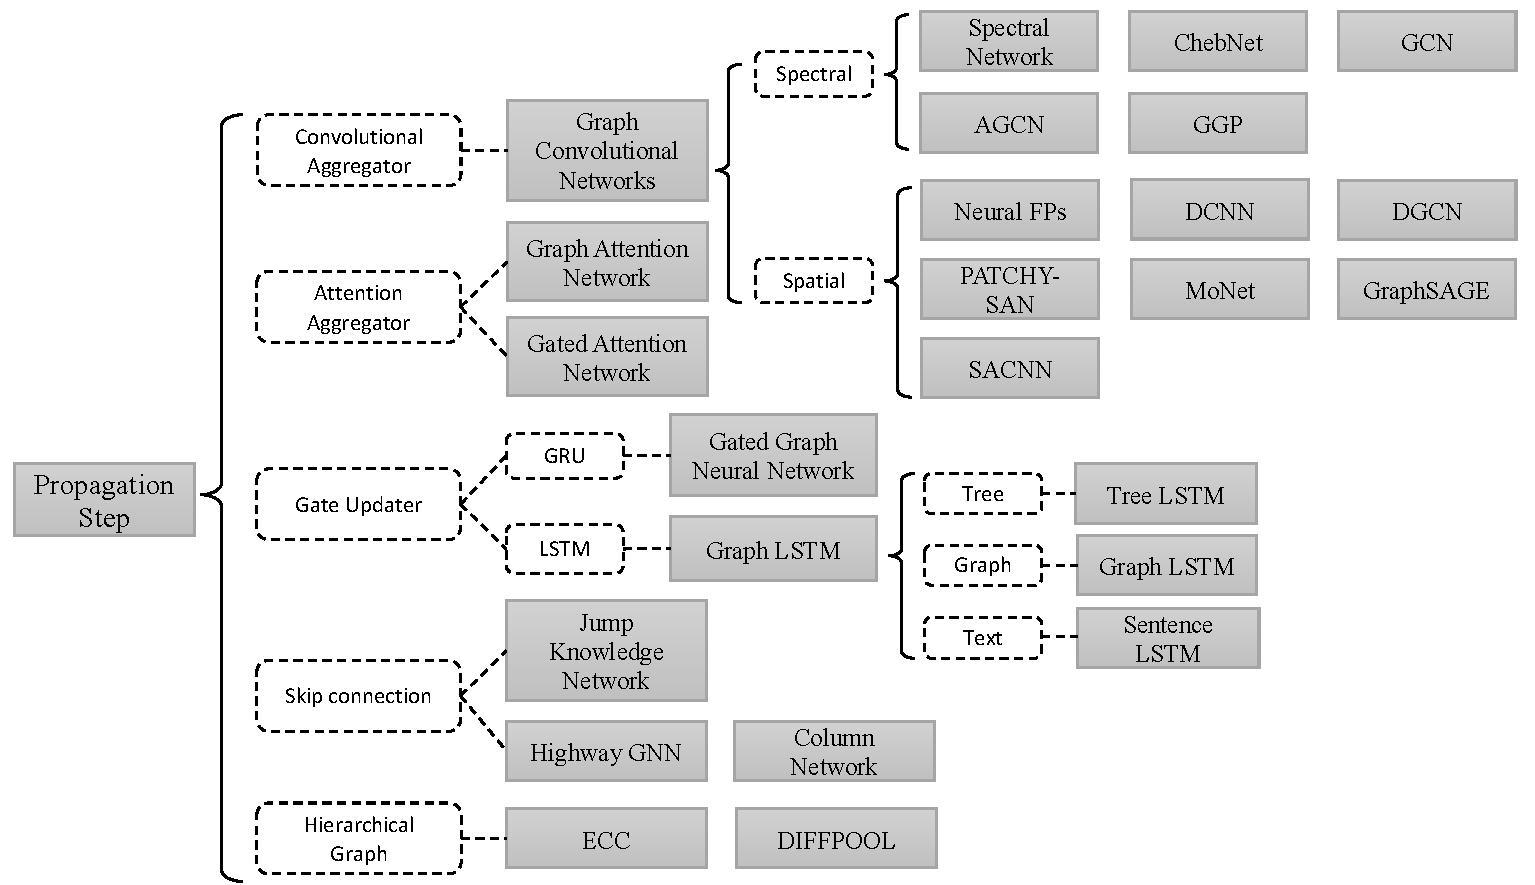
\includegraphics[width=1\linewidth]{images/GNN-variants/variant2.pdf}
		\end{subfigure}
	\end{figure}\footnote{\cite{zhou_graph_2019}}
\end{frame}

\section{DeepWalk}

\begin{frame}{DeepWalk 1}
	\begin{itemize}
		\item Inspirována metodami word2vec a skip-gram z NLP.
		\item Náhodné procházky z daného vrcholu (\( M \) procházek délky \( L \))
	\end{itemize}
\end{frame}

\begin{frame}{DeepWalk 2}
	\centering
	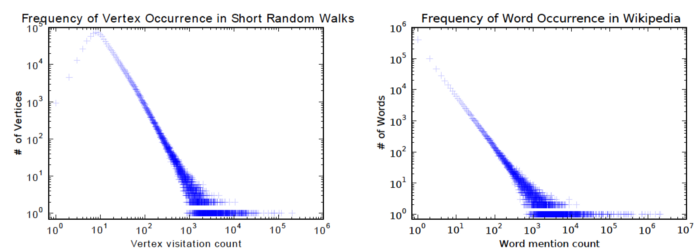
\includegraphics[width=0.8\pagewidth]{images/DeepWalk-word2vec.png}\footnote{\cite{perozzi_deepwalk_2014}}
\end{frame}

\begin{frame}{DeepWalk -- skip-gram}
	\centering
	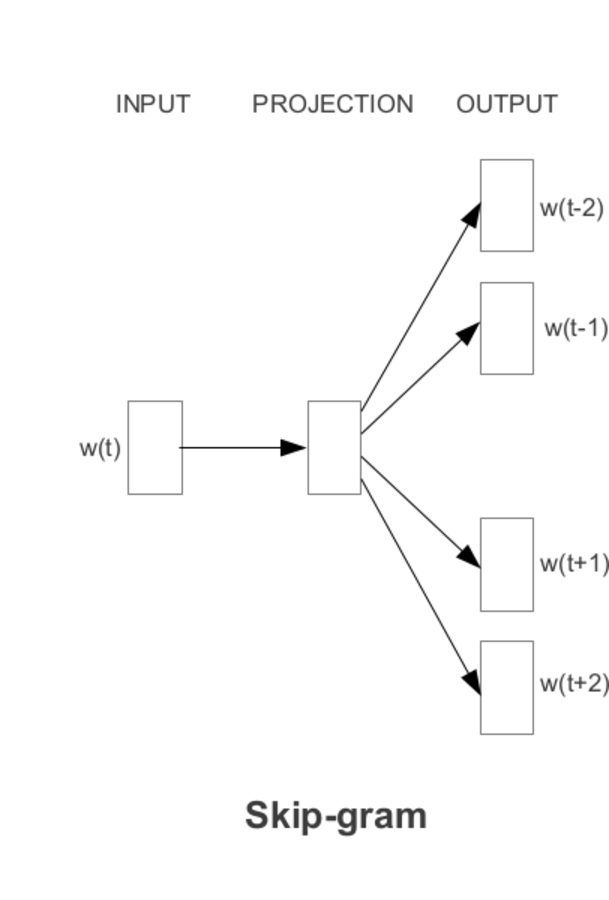
\includegraphics[width=0.4\pagewidth]{images/SkipGram.pdf}\footnote{\cite{mikolov_efficient_2013}}
\end{frame}

\begin{frame}{DeepWalk 4}
	\begin{itemize}
		\item Pro každý vektor \( v \) učíme jeho reprezentaci \( f : \mathspace{V} \to \mathfield{R}^{\left\lvert \mathfield{V} \right\rvert \times d} \)
		\item Snažíme se maximalizovat hodnotu
			\[ \mathrm{P} \left( \left\{ v_{i - w}, \dots, v_{i + w} \right\} \setminus v_i \middle| f \left( v_i \right) \right) \]
		\item Za předpokladu nezávislosti zjednodušíme
			\[ \mathrm{P} \left( \left\{ v_{i - w}, \dots, v_{i + w} \right\} \setminus v_i \middle| f \left( v_i \right) \right) = \prod_{\substack{j = i - w \\ j \neq i}}^{i + w} \mathrm{P} \left( v_j \middle| f \left( v_i \right) \right) \]
		\item Je třeba dále zefektivnit pomocí hierarchical softmax.
	\end{itemize}
\end{frame}

\begin{frame}{DeepWalk -- závěr}
	\begin{itemize}
		\item Použití myšlenek word2vec pro učení se na grafech.
		\item Neumí klasifikovat nové vrcholy - je třeba přetrénovat model.
	\end{itemize}
\end{frame}

\section{node2vec}

\begin{frame}{node2vec 1}
	\begin{itemize}
		\item Inspirována metodou word2vec z NLP.
		\item Hledáme embedding \( \mathrm{node2vec} : \mathspace{G} \to \mathfield{R}^n \).
	\end{itemize}
\end{frame}

\begin{frame}{node2vec 2}
	\centering
	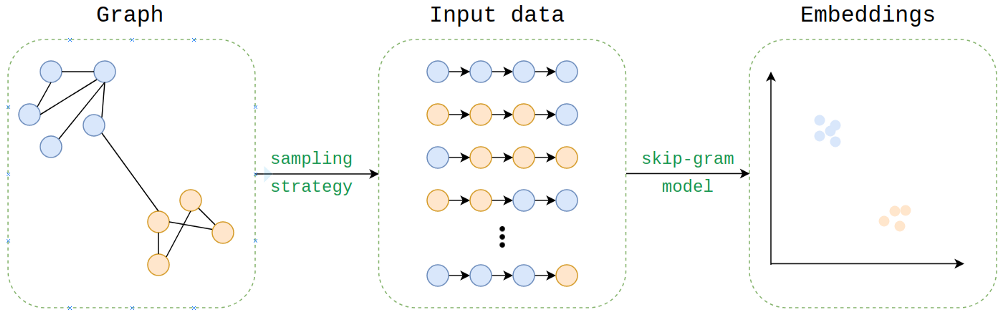
\includegraphics[width=0.9\pagewidth]{images/node2vec.png}\footnote{\cite{cohen_node2vec_2018}}
\end{frame}

\begin{frame}{node2vec 3}
	\begin{itemize}
		\item Pro každý vektor \( v \) učíme jeho reprezentaci \( f : \mathspace{V} \to \mathfield{R}^{\left\lvert \mathfield{V} \right\rvert \times d} \)
		\item Snažíme se maximalizovat hodnotu
			\[ \mathrm{P} \left( ne \left[ v \right] \middle| f \left( v \right) \right) \]
		\item Za předpokladu nezávislosti zjednodušíme
			\[ \mathrm{P} \left( ne \left[ v \right] \middle| f \left( v \right) \right) = \prod_{v_i \in ne \left[ v \right]} \mathrm{P} \left( v_i \middle| f \left( v \right) \right) \]
		\item Je třeba dále zefektivnit pomocí hierarchical softmax a negative sampling.
	\end{itemize}
\end{frame}

\begin{frame}{node2vec 4}
	\begin{itemize}
		\item Jak hledat \( ne \left[ v \right] \)?
		\item 2 extrémy: BFS, DFS
		\item Běžná náhodná procházka: Jsem-li ve vrcholu \( v \), jdu do nějakého vrcholu spojeného s \( v \), se stejnou pravděpodobností pro všechny takové vrcholy.
		\item Upravíme náhodnou procházku, aby interpolovala mezi BFS a DFS.
		\item Pokud jsme právě přišli z vrcholu \( t \) do vrcholu \( v \) a zvažujeme, kam jít dál, všem kandidátům \( x \) přiřadíme váhu
			\[ \alpha \left( t, x \right) = \begin{cases}
				\frac{1}{p} &\text{ pro } d_{tx} = 0 \\
				1 &\text{ pro } d_{tx} = 1 \\
				\frac{1}{q} &\text{ pro } d_{tx} = 2 \\
			\end{cases} \]
			kde \( d_{tx} \) je délka nejkratší cesty z \( t \) do \( x \) a \( p, q \) jsou parametry modelu.
	\end{itemize}
\end{frame}

\begin{frame}{node2vec 5}
	\centering
	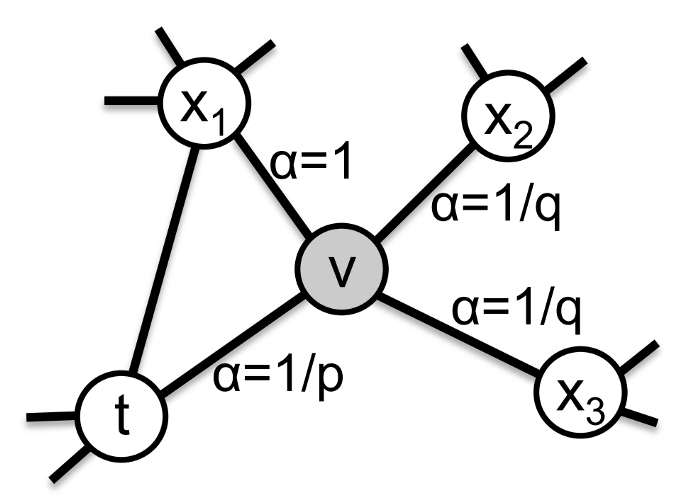
\includegraphics[width=0.7\pagewidth]{images/node2vec-alpha.png}\footnote{\cite{grover_node2vec_2016}}
\end{frame}

\begin{frame}{node2vec -- závěr}
	\begin{itemize}
		\item Použití myšlenek word2vec pro učení se na grafech.
		\item Vylepšení DeepWalk
		\item Neumí klasifikovat nové vrcholy - je třeba přetrénovat model.
	\end{itemize}
\end{frame}

\section{GCN}

\begin{frame}{GCN 1}
	\begin{itemize}
		\item Řešíme úlohu \enquote{Node classification}.
		\item Inspirována konvolučními neuronovými sítěmi.
	\end{itemize}
\end{frame}

\begin{frame}{GCN 2}
	\begin{itemize}
		\item Vyjádření neuronové sítě operující na celém grafu, podobně jako u GNN.
		\item Každá vrstva je tvaru
			\[ \mathmat{H}^{l + 1} = f \left( \mathmat{H}^{(l)}, \mathmat{A} \right) \]
			kde \( \mathmat{A} \) je adjacenční matice.
		\item Můžeme vyjádřit jednoduchou vrstvu jako
			\[ f \left( \mathmat{H}^{(l)}, \mathmat{A} \right) = \sigma \left( \mathmat{A} \mathmat{H}^{(l)} \mathmat{W}^{(l)} \right) \]
			kde \( \mathmat{W} \) jsou váhy a \( \sigma \) aktivační funkce.
	\end{itemize}
\end{frame}

\begin{frame}{GCN 3}
	\begin{itemize}
		\item Abychom v každém kroku kromě sousedů vrcholu uvažovali i vrchol samotný, použijeme místo \( \mathmat{A} \) matici \( \widehat{\mathmat{A}} = \mathmat{A} + \mathmat{I} \).
		\item Protože matice \( \mathmat{A} \) není normalizovaná, měnila by se nám škála po každé vrstvě. Abychom tomu zabránili, použijeme místo \( \mathmat{A} \) symetricky normalizovanou matici \( \mathmat{D}^{-\frac{1}{2}} \mathmat{A} \mathmat{D}^{-\frac{1}{2}} \) kde \( \mathmat{D} \) je disgonální matice stupňů jednotlivých vrcholů.
		\item Dostáváme tedy vrstvu sítě jako
			\[ f \left( \mathmat{H}^{(l)}, \mathmat{A} \right) = \sigma \left( \widehat{\mathmat{D}}^{-\frac{1}{2}} \widehat{\mathmat{A}} \widehat{\mathmat{D}}^{-\frac{1}{2}} \mathmat{H}^{(l)} \mathmat{W}^{(l)} \right) \]
	\end{itemize}
\end{frame}

\begin{frame}{GCN 4}
	\centering
	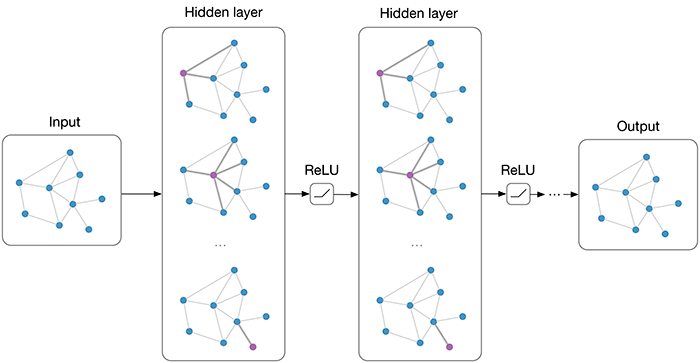
\includegraphics[width=0.8\pagewidth]{images/GCN.png}\footnote{\cite{kipf_how_2016}}
\end{frame}

\begin{frame}{GCN -- závěr}
	\begin{itemize}
		\item Použití myšlenek CNN pro učení se na grafech.
		\item GCN jsou aproximací prvního řádu lokálních spektrálních filtrů na grafech - viz \cite{kipf_semi-supervised_2017}.
	\end{itemize}
\end{frame}

\begin{frame}{GraphSAGE 1}
	\begin{itemize}
		\item GraphSAGE je induktivní metoda -- tedy nepotřebuje při učení znát celý graf.
		\item Učíme se reprezentaci vektoru \( v \) pomocí reprezentací jeho sousedů, tj.
			\[ \mathvec{h}_v^{(l + 1)} = \sigma \left( \mathmat{W}^{(l)} \cdot \mathrm{concat} \left( \mathvec{h}_v^{(l)}, \mathvec{h}_{ne \left[ v \right]}^{(l)} \right) \right) \]
			kde
			\[ \mathvec{h}_{ne \left[ v \right]}^{(l)} = \textsc{aggregate}_l \left( \left\{ h_u^{(l)} \middle| u \in ne \left[ v \right] \right\} \right) \]
		\item Potřeba učit speciální ztrátovou funkcí.
	\end{itemize}
\end{frame}

\begin{frame}{GraphSAGE 2}
	\centering
	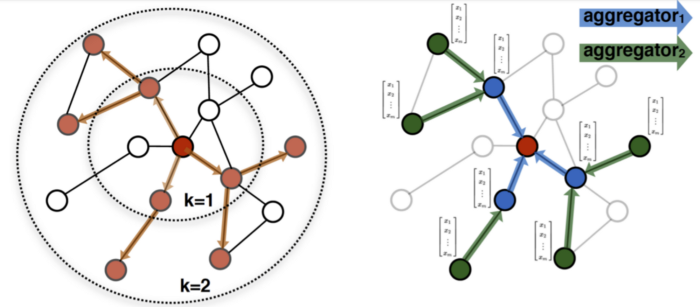
\includegraphics[width=0.7\pagewidth]{images/GraphSAGE.png}\footnote{\cite{hamilton_inductive_2017}}
\end{frame}

\begin{frame}{GraphSAGE 3}
	\begin{itemize}
		\item Máme volbu agregátorů v každé vrstvě
		\item Aritmetický průměr po složkách vede na vrstvy typu GCN.
		\item LSTM agregátor (musíme náhodně permutovat sousedy)
		\item Pooling:
			\[ \textsc{aggregate}_l = \max \left\{ \sigma \left( \mathmat{W}_{\mathrm{pool}} \mathvec{h}_u^{(l)} + \mathvec{b} \right) \middle| u \in ne \left[ v \right] \right\} \]
	\end{itemize}
\end{frame}

\begin{frame}{GraphSAGE -- závěr}
	\begin{itemize}
		\item Induktivní přístup se hodí pro grafy, do kterých po tréninku přibývají vrcholy.
		\item Nemusíme přepočítávat model, bude fungovat i s novými daty.
	\end{itemize}
\end{frame}

\begin{frame}
	\centering
	
\includegraphics[width=0.75\pagewidth]{images/thats-all.png}
\end{frame}

\begin{frame}[allowframebreaks]{Zdroje}
	\printbibliography
\end{frame}

\end{document}
